\documentclass[a4paper, 12pt]{article}
\usepackage[english]{babel}
\usepackage[left=2.5cm, right=2.5cm, top=2.5cm, bottom=2.5cm]{geometry}
\usepackage{natbib}
\usepackage{listings}
\usepackage{url}
\usepackage{wrapfig}
\usepackage[utf8x]{inputenc}
\usepackage{amsmath}
\usepackage{graphicx}
\graphicspath{{images/}}
\usepackage{parskip}
\usepackage{fancyhdr}
% \usepackage{vmargin}
\usepackage{caption}
\usepackage{color}
 
\definecolor{codegreen}{rgb}{0,0.6,0}
\definecolor{codegray}{rgb}{0.5,0.5,0.5}
\definecolor{codepurple}{rgb}{0.58,0,0.82}
\definecolor{backcolour}{rgb}{0.95,0.95,0.92}

\lstdefinestyle{mystyle}{
    backgroundcolor=\color{backcolour},   
    commentstyle=\color{codegreen},
    keywordstyle=\color{magenta},
    numberstyle=\tiny\color{codegray},
    stringstyle=\color{codepurple},
    basicstyle=\scriptsize,
    breakatwhitespace=false,         
    breaklines=true,                 
    captionpos=b,                    
    keepspaces=true,                 
    numbers=left,                    
    numbersep=5pt,                  
    showspaces=false,                
    showstringspaces=false,
    showtabs=false,                  
    tabsize=2
}
 
\lstset{style=mystyle}

\title{Midterm 1 - Project CTE Document}
\author{Nasir Mohammad Khalid}
\date{March 4, 2019}

\makeatletter
\let\thetitle\@title
\let\theauthor\@author
\let\thedate\@date
\makeatother

\begin{document} 
    \begin{titlepage}
        \centering
        \vspace*{0.5 cm}
        
\includegraphics[scale = 0.60]{logo.png}\\[1.0 cm]	% University Logo
        \textsc{\LARGE American University of Sharjah}\\[1.0 cm]
        \textsc{\Large ELE494-08}\\[0.2 cm]	
        \textsc{\Large Autonomous robotic systems}\\[0.5 cm]			% Course Code
        \rule{\linewidth}{0.2 mm} \\[0.4 cm]
        { \huge \bfseries \thetitle}\\
        \rule{\linewidth}{0.2 mm} \\[1.5 cm]
        
        \textsc{\Large{\theauthor}}\\[0.3 cm]
        \textsc{\Large{65082}}\\[0.3 cm]
        \textsc{\Large{\thedate}}\\[1.5 cm]

        \textmd{Submitted To: \itshape{Dr.Shayok Mukhopadhyay}}
    \end{titlepage}

    \clearpage
    \tableofcontents
    \listoffigures
    \listoftables
    \clearpage

    \section{Initial Goal Statement}

    The goal of our group project is to create a robot which will navigate in a region while avoiding obstacles to find the spot with the most sunlight.

    \section{Team Formation}

    For the project my group member is Yousif Khaireddin (@63618). We have worked together previously as lab partners and on projects in other courses. Therefore, we understand each others strengths/weaknesses and since our hobbies are quite similar it is easier for us to get along. 

    Youssif got in touch with me during our class and we decided to form the group and discuss what timings we have to work on the project.

    \begin{figure}[h]
        \centering
        \captionsetup{justification=centering}
        \centering
            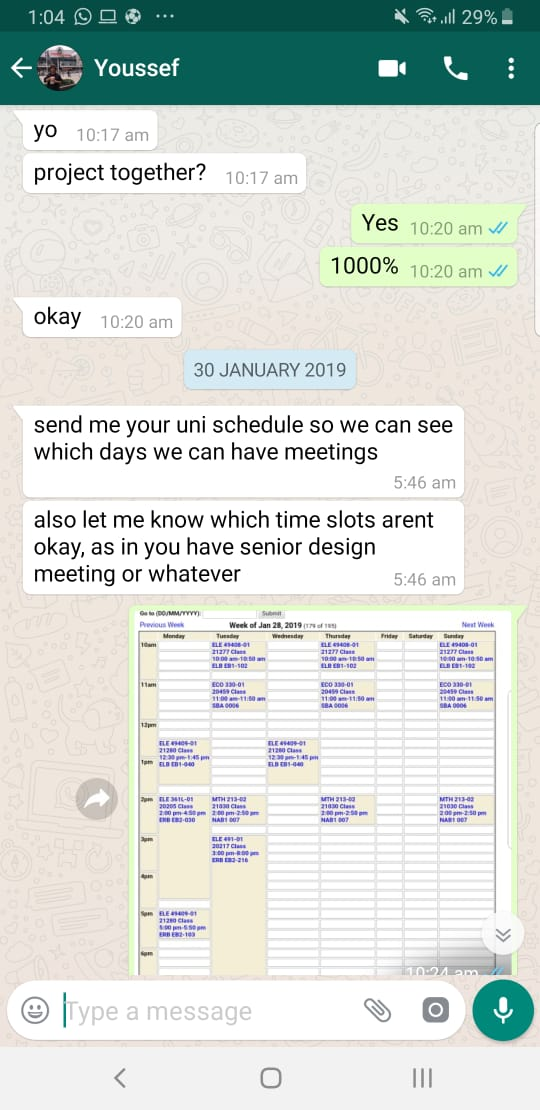
\includegraphics[width=0.3\textwidth]{GF.jpeg}
            \caption{Forming group and planning meetings}
    \end{figure}


    After this we decided to have meetings on Thursday after 3 pm and during this time we will work on the project.

    \subsection{First Meeting}

    Our first meeting took place in the library and during it we brainstormed on possible ideas for what the project will be. At the end we had a list of projects that we thought were suitable and these included:

    \begin{itemize}
        \item Drink Pouring Machine
        \item Light Detection for Solar Panels
        \item A Plotter that could draw shapes
        \item Robot that will follow the path of a line on the floor
        \item A software simulation of a robot that will stay in lane
    \end{itemize}

    We then arranged for a meeting with Dr.Shayok and through the discussion we decided on developing a robot that can move freely within a region while avoiding obstacles and at the end of its journey it returns to tell the user the location with the brightest sunlight.

    \begin{figure}[h]
        \centering
        \captionsetup{justification=centering}
        \centering
            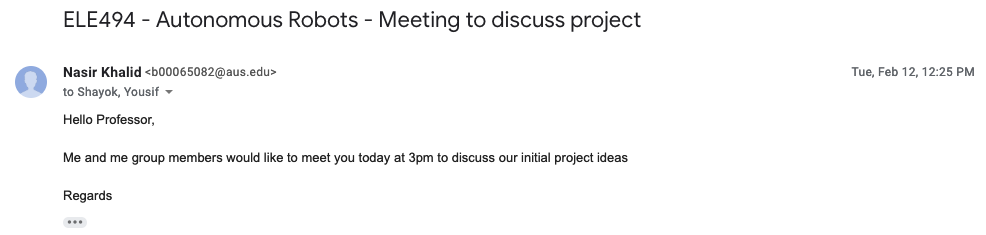
\includegraphics[width=0.8\textwidth]{M1}
            \caption{Arranging First Meeting with Professor}
    \end{figure}

    \subsection{Meeting 2}

    During our second meeting me and Youssif discussed how we could realize the project goal. We ultimately decided that we would 
    create a physical robot and through our discussions we planned some of the basic circuitry and also placed orders for the components needed.

    \begin{figure}[h]
        \centering
        \captionsetup{justification=centering}
        \centering
            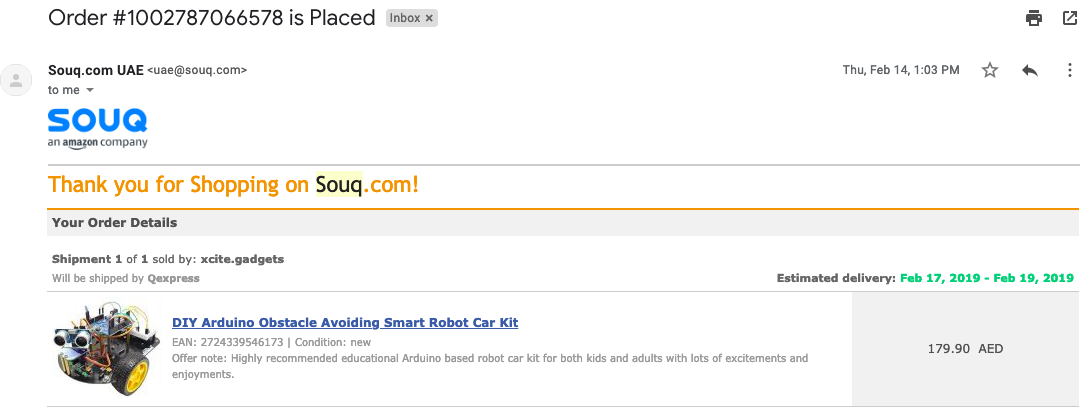
\includegraphics[width=0.6\textwidth]{Order}
            \caption{Ordering the robot components}
    \end{figure}

    \begin{figure}[h]
        \centering
        \captionsetup{justification=centering}
        \centering
            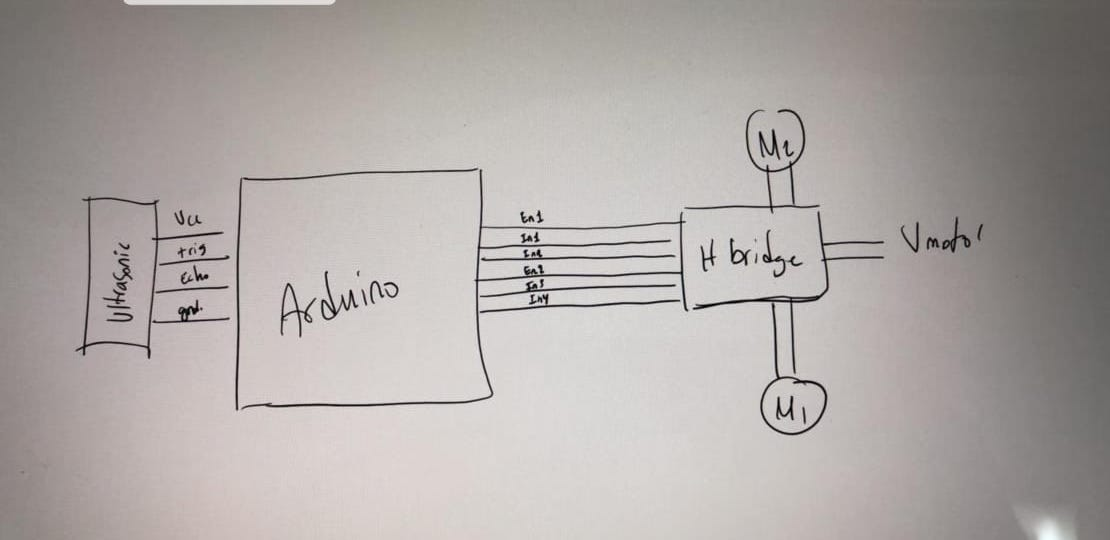
\includegraphics[width=0.5\textwidth]{Circuit}
            \caption{Understanding the connections needed}
    \end{figure}

    \subsection{Subsequent Meetings}

    Once the components arrived we met again multiple times to begin assembly and testing
    of the components we recieved. We both worked together in building the frame and assembling the components. Yousif focused on the wiring of all the components

    However, when it came to testing we split the software work between us. Youssif developed the code for testing the Ultrasonic sensor and I developed the code to test the motors and servo.

    Shown below are snippets of testing code used for the motor and servo.

    \begin{lstlisting}[language=C++, caption=MotorTest Code]
    #include <L298N.h>

    //pin definition
    #define EN 9
    #define IN1 8
    #define IN2 7
    #define EN2 3
    #define IN3 1
    #define IN4 2

    int speed1 = 0;

    void setup() {
    pinMode(EN1, OUTPUT);
    pinMode(IN1, OUTPUT);
    pinMode(IN2, OUTPUT);
    pinMode(EN2, OUTPUT);
    pinMode(IN3, OUTPUT);
    pinMode(IN4, OUTPUT);
    }

    void loop() {
    //  The following code tests the motors by speeding them up slowly
    //  and then bringing speeds back down to zero
    if(speed1 == 255){
        speed1 = 0;
    }
    
    analogWrite(EN1, speed1);
    analogWrite(EN2, speed1);
    digitalWrite(IN1, HIGH);
    digitalWrite(IN2, LOW);
    digitalWrite(IN3, HIGH);
    digitalWrite(IN4, LOW);
    delay(500);
    speed1 += 10;
    }\end{lstlisting}  

    \begin{lstlisting}[language=C++, caption=ServoTest Code]
    #include <Servo.h>
    #define SERVO_PIN 9
    Servo myservo;     
    int pos = 0;
    
    void setup() {
        myservo.attach(SERVO_PIN); 
    }
    
    void loop() {
        //Sweeps the entire servo head. Looking left to right
        for (pos = -180; pos <= 180; pos += 1) {
        myservo.write(pos);              
        delay(15);                     
        }
    }\end{lstlisting}

    After our testing we then met with Dr.Shayok again to discuss on how we can use the encoders going forward. We also placed the order for these encoders and once they arrive we expect to continue work on the project. 

    \begin{figure}
        \centering
        \captionsetup{justification=centering}
        \centering
            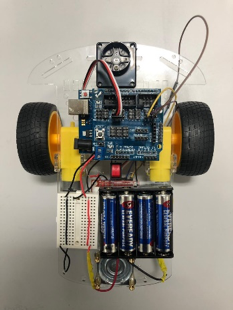
\includegraphics[width=0.3\textwidth]{robot_up.png}
            \caption{Top side of the robot}
    \end{figure}

    \begin{figure}
        \centering
        \captionsetup{justification=centering}
        \centering
            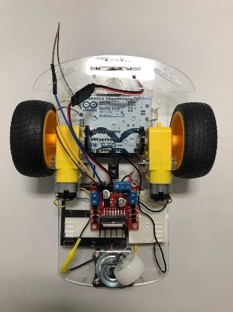
\includegraphics[width=0.3\textwidth]{robot_down.png}
            \caption{Bottom side of the robot}
    \end{figure}

    \section{Team strengths and weaknesses assessment}

    \begin{table}[h!]
        \centering
        \begin{tabular}{l|l|l|}
        \cline{2-3}
                                                           & \multicolumn{1}{c|}{\textit{\textbf{Nasir}}}                                                                      & \multicolumn{1}{c|}{\textit{\textbf{Youssif}}}                                                                             \\ \hline
        \multicolumn{1}{|c|}{\textit{\textbf{Strengths}}}  & \begin{tabular}[c]{@{}l@{}}- Experienced with Arduino\\ - Programming\\ - More free time in schedule\end{tabular} & \begin{tabular}[c]{@{}l@{}}- Better at developing circuitry\\ - Programming\\ - Handy work\\ - Lives in dorms\end{tabular} \\ \hline
        \multicolumn{1}{|l|}{\textit{\textbf{Weaknesses}}} & - Procrastination                                                                                                 & \begin{tabular}[c]{@{}l@{}}- Time Management\\ - Doing multiple projects this semester\end{tabular}                        \\ \hline
        \end{tabular}
        \caption{Strength and weaknesses assessment}
        \label{my-label}
    \end{table}

    \section{Team Member Roles}

    Currently as we are in the early stages of the project and developing the ground work, we have not yet split our roles and seperated tasks.
    However, as we progress further it is becoming quite clear that we will be splitting up and each working on a seperate part of the robot which will ultimately come together and lead to our final project.

    For the work done until now the roles can be seen in the table below: 

    \begin{table}[h]
        \resizebox{\textwidth}{!}{%
        \begin{tabular}{|l|l|}
        \hline
        \multicolumn{1}{|c|}{\textit{\textbf{Nasir}}}                                                                                                                                                 & \multicolumn{1}{c|}{\textit{\textbf{Youssif}}}                                                                                                                                                            \\ \hline
        \begin{tabular}[c]{@{}l@{}}- Assembling the Robot\\ - Soldering all wires in place\\ - Ordering and identifying components needed\\ - Writing test code for different components\end{tabular} & \begin{tabular}[c]{@{}l@{}}- Assembling the Robot\\ - Figuring out where to place components on the chasis\\ - Developing circuitry for robot\\ - Writing test code for different components\end{tabular} \\ \hline
        \end{tabular}%
        }
        \caption{My caption}
        \label{my-label}
    \end{table}

    As we go forward we will be splitting the different functions of the robot between ourselves along with the tasks that come up.

    \section{Broad Objectives}

    Our end goal is that our robot will be able to move within any region while avoiding obstacles and it will also be able to return and inform the user about the brightest spot it finds.
    This entire project can be split in to two sections:

    \begin{itemize}
        \item Moving freely on ground while avoiding obstacles
        \item Storing light intensity data across the area it travels
    \end{itemize}

    We require encoders and a gyroscopic sensor along with the knowledge of path planning to fully realize the first item on the list. For the second item we are trying to develop a method of measuring total light intensity in 3D space so as to find the brightest spot. Currently our robot is capable of moving and through the Ultrasonic sensor + Servo
    we are able to detect obstacles in it's path. Once we discuss certain topics in the course and recieve the remaining components we will move forward.

    Such a robot seems practical for real world applications. In one case it could give solar powered vehicles the ability to charge themselves by navigating obstacles and finding the area with the most light intensity.
\end{document}